% !TEX root =  manuscript.tex
\subsection{Trends and Landscape}\label{sec:trends}

\begin{figure}%[b]
	\revised{\linewidth}{
		\centering
		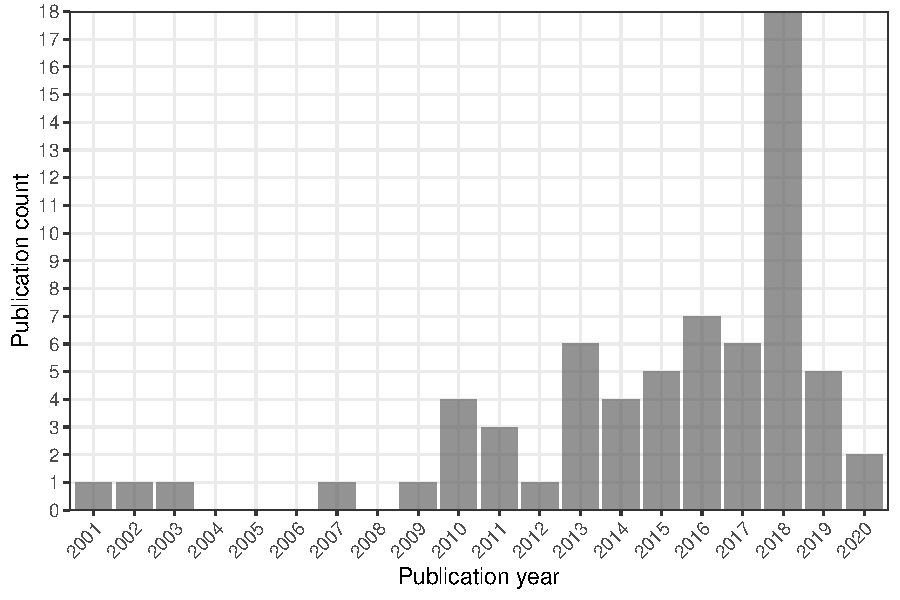
\includegraphics[width=0.85\textwidth]{survey/figures/years-publications}
		\caption{Distribution of publications across years. }
		\label{fig:years-publications}
	}
\end{figure}


\changed{
At the end of the paper collection process,
we obtained a pool of papers spanning the years 2001-2020 (June 2020).
\autoref{table:selected-primary-studies} shows
the final list of \numberOfPapers papers.
\autoref{fig:years-publications} shows the distribution of
the retrieved pool of papers across different years of publication.
Overall, we observed a generally increasing long-term trend in
the use of computer vision approaches in software engineering. 
This research area is also relatively new, 
with more than half of the papers in our pool 
published in the past five years.
Furthermore, \autoref{fig:areas-trend} depicts the cumulative number of publications 
per software engineering area across different years.
The results indicate that software testing is the area 
exhibiting the most rapid increase
in terms of the number of publications 
wherein a computer vision technique is utilized.
}




\begin{figure}
\revised{\linewidth}{
\centering
%\fbox{
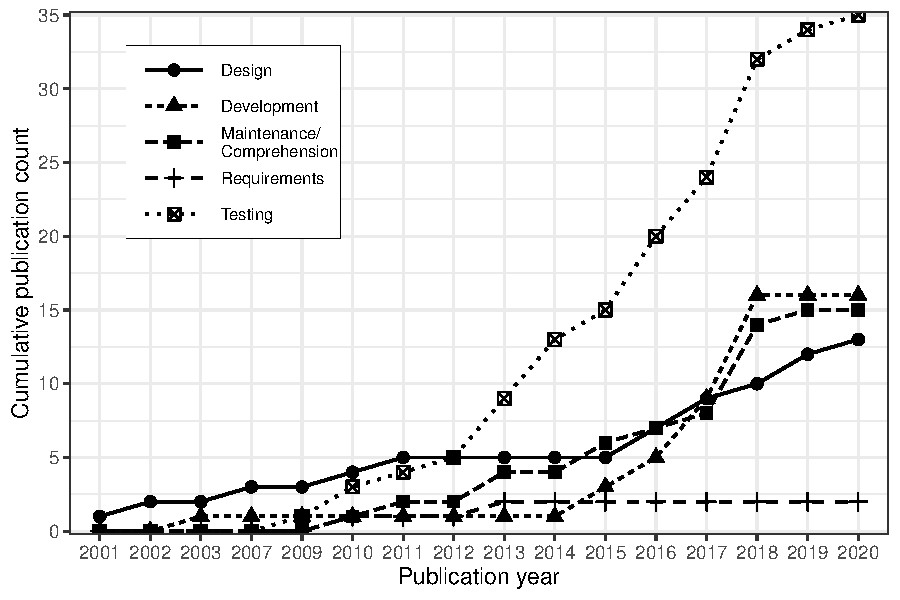
\includegraphics[width=\linewidth]{survey/figures/areas-trend-cumulative}
%}
\caption{Cumulative distribution of publications across years per SE area.
Testing is the most common area, followed by development and maintenance.} \label{fig:areas-trend} 
}
\end{figure}

\changed{
\autoref{fig:venues-publications} shows the distribution 
of the published papers across venues.
The main venues in which computer vision approaches 
for software engineering were published are 
the Conference on Human Factors in Computing Systems (CHI) with 11 papers, 
the International Conference on Software Engineering (ICSE) with nine papers, 
and the International Conference on Automated Software Engineering (ASE) with eight papers. 
The presence of traditional SE venues as well as venues from other fields (e.g. CHI) 
in \autoref{fig:venues-publications} provides some indication that 
research on the use of computer vision for software engineering tasks 
is an interdisciplinary field. 
}


\subsection{Areas, Tasks, and Platforms (RQ1)}\label{sec:rq1}

\begin{figure}%[b]
	\revised{\linewidth}{
		\centering
		%\fbox{
		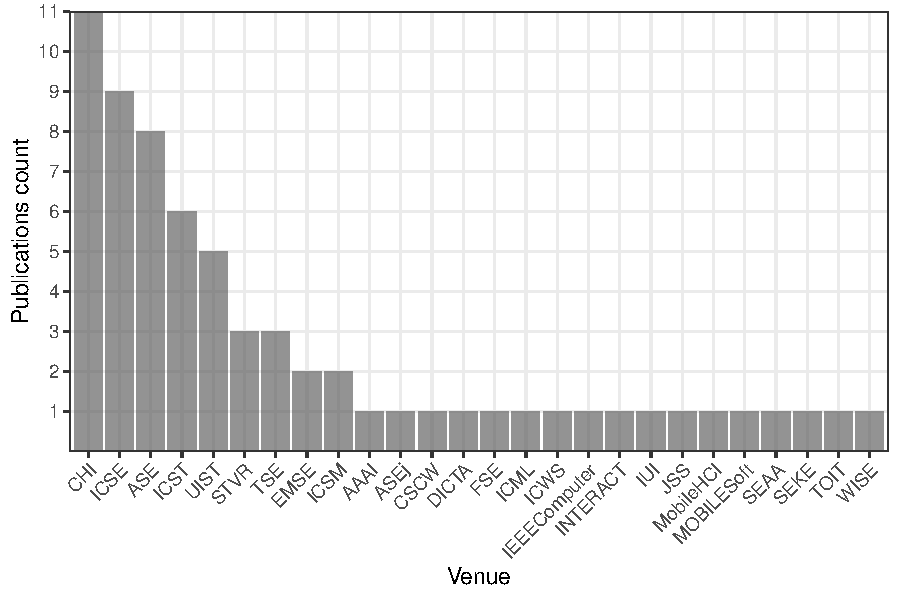
\includegraphics[width=\linewidth]{survey/figures/venues-publications}
		%}
		\caption{Distribution of the publications across venues. }\label{fig:venues-publications}
	}
\end{figure}

To study the exiting applications of visual techniques for SE,
we analyzed the selected papers to find out
which \textit{SE areas} have been explored,
for which \textit{tasks}, and on which \textit{platforms} they were used.
As defined in section \ref{sec:defs}, SE areas are high-level stages
of the software engineering life cycle,
such as requirements, testing, or development.
SE tasks are more fine-grained activities, such as unit testing or regression testing.
The platforms are the types of computing devices (e.g., desktop, mobile) 
that the analyzed software runs on. 
We further looked into the papers' discussion sections to gain insights from
the authors about other areas in which the proposed technique could potentially be applied.

\subsubsection{Software Engineering Areas and Tasks}

\autoref{fig:software-engineering-tasks}
presents the papers distribution across different SE areas and tasks.
Note that the number of papers indicated in the figure
is more than the total number of papers in the pool.
This is due to the fact that for some papers, the presented approach can be utilized for more than one task.
We now discuss more in detail the trends of \autoref{fig:software-engineering-tasks}.

\begin{figure}
    \revised{\linewidth}{
\centering
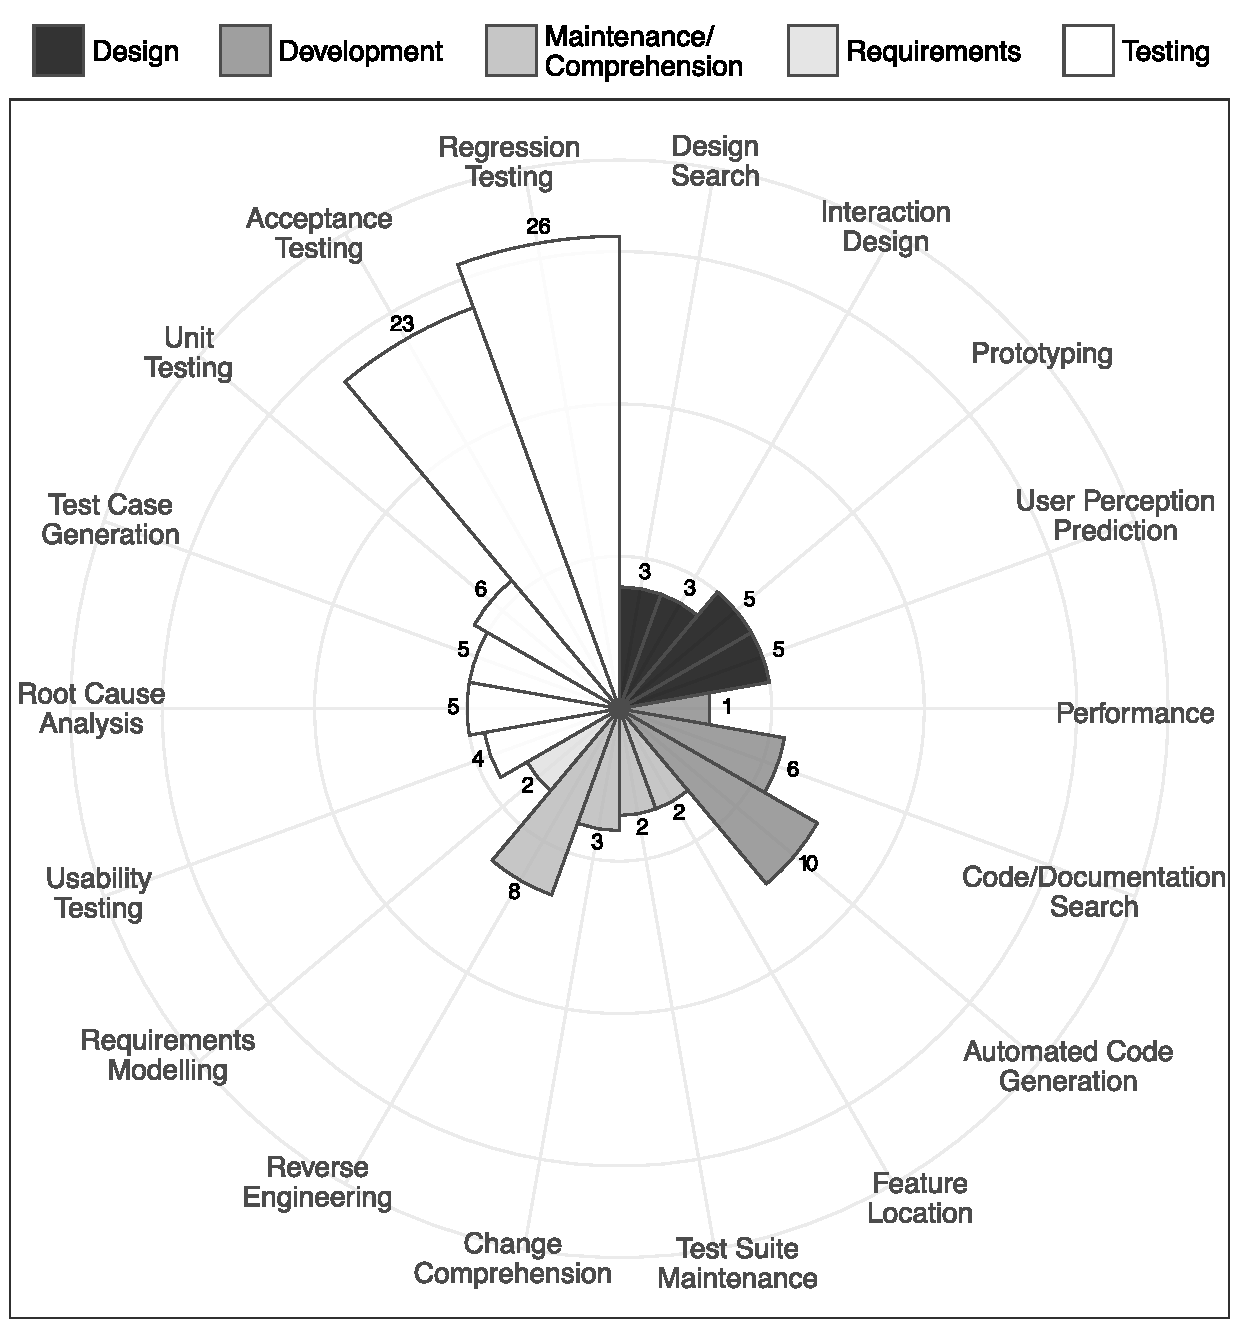
\includegraphics[width=0.8\linewidth]{survey/figures/areas}
\caption{Papers distribution across different Software Engineering Areas and Tasks}
\label{fig:software-engineering-tasks}
    }
\end{figure}


\header{Testing}
Software testing is the most common research area 
for which approaches using computer vision are proposed, 
accounting for approximately half of all collected papers.
A closer look at the publications in this area reveals interesting trends. 
\textbf{Regression Testing.} Most of the studies use visual methods to facilitate acceptance and regression testing e.g., by 
comparing visual artifacts (e.g., the GUIs) 
with each other or with respect to a given oracle.
Without adopting computer vision, developers would most 
likely need to perform some kind of manual evaluation, 
e.g., through eyeball analysis to spot deviations from 
the expected visual presentation---a daunting and error-prone task.
Apart from GUI comparisons, computer vision (CV) techniques have been also utilized 
for other software testing tasks.
%
For example,
%
\citet{Kuchta-2018-EMSE} introduce a technique for regression 
testing of PDF reader software and localizing faulty parts of PDF files.
The adopted technique exploits \textit{differential testing}, 
where the (visual) output of multiple implementations of a 
program---the PDF viewer---is compared to the same input to spot deviations.
%
In another work, \citet{Leotta-2018-STVR} propose an automated 
code migration tool for automatically converting end-to-end 
Selenium web tests to visual web tests based on 
Sikuli's~\cite{Chang-2010-CHI} image recognition capabilities.
%
\citet{Kirac-2018-JSS} provide an image comparison technique 
for black-box, regression testing of visual-output software 
used in consumer electronics.
The approach removes noise to eliminate image differences 
caused by scaling and translation, and is evaluated on the output of digital TVs.
%
\citet{canvas_icst2018} propose a technique to test 
state-free canvas elements on web pages by reverse-engineering a visual model.
This allows unit testing of the specific visual elements contained in the canvas.


\textbf{Cross-browser Testing}. A significant class of software testing techniques leveraging visual methods aims at automatically identifying \textit{cross-browser incompatibilities} (XBIs) for web 
applications~\cite{Choudhary-2010-ICSM, Choudhary-2012-ICST,
Semenenko-2013-ICSM, Choudhary-2013-ICSE, Selay-2014-DICTA, He-2016-ICWS, Xu-2018-TOIT}.
XBIs are frequently-occurring issues in web pages' 
appearance and/or behavior when the same page is viewed 
on different web browsers~\cite{Choudhary-2013-ICSE}.
Identifying such differences requires laborious human judgement,
which can be effectively reduced using an automated visual-based technique.
A recent literature review by \citet{Sabaren-2018-JCST} 
surveys the techniques proposed to tackle XBIs.

A similar problem involves using visual methods for 
\textit{root cause analysis} of presentational issues 
occurring on web pages~\cite{Mahajan-2014-ASE, Mahajan-2015-ICST,
Mahajan-2016-ICST}.
In addition to the web domain, root cause analysis 
is also used to identify rendering issues in PDF 
files~\cite{Kuchta-2018-EMSE}, as well as, the causes
of excessive energy consumption of UIs in mobile 
applications~\cite{Wan-2017-STVR}.

Several approaches attempt to automate test 
execution using visual techniques. An example 
is \textit{record-and-replay testing} where the 
screenshots of the GUI and the human tester's 
actions and inputs performed on the GUI are recorded~\cite{Chang-2010-CHI,
Alegroth-2013-ICST, Lin-2014-TSE, He-2016-ICWS} . 
Popular visual record-and-replay tools are 
Sikuli~\cite{Chang-2010-CHI} and 
JAutomate~\cite{Alegroth-2013-ICST}, which allow 
fast and easy replay of the same sequence of actions:
the tool conducts a visual search on the current 
visible contents of the screen to detect the 
widgets' locations, triggers the recorded 
actions and inputs, and finally performs a visual assertion,
comparing the observed visual outcome with the expected oracle.

Besides record-and-replay tools, test automation with 
visual analysis has been successfully applied to 
\textit{automotive software engineering}. 
\citet{Amalfitano-2014-WISE} propose a tool to automate 
the testing of the emulated vehicle information 
systems' panels.
The testers can locate visual elements on the panel 
and specify their properties; the tool allows to 
check the panel's output with respect to these 
properties at pre-defined timestamps.

\changed{
\citet{Zheng-2009-CHI}, \citet{Yuan-2020-CHI}, 
\citet{Deka-2016-UIST}, and \citet{Deka-2017-UIST} 
aim to automate the testing of \textit{aesthetics 
or usability} of web pages. 
This line of work involves building computer vision 
models that can predict whether web pages 
meet certain aesthetic requirements pertaining to 
the usability of a page (e.g. visual balance of 
white space and elements, consistent and simple 
representation of elements on a web page).
}

\citet{Patric-2016-ASE} propose an approach based 
on systematic image manipulation to \textit{automatically 
generate test input images} for regression and 
acceptance testing of an epidemiological simulation software.
The software's output on these input images is 
monitored and unexpected deviations reveal bugs or regressions in the code.

To \textit{prioritize test reports}, \citet{Feng-2016-ASE} 
use the screenshots provided by users to augment the 
existing textual test prioritization techniques for mobile applications. 
Finally, to \textit{automatically generate test cases}, 
\citet{Zhang-2017-ASE} use a visual-aided approach
that identifies strokes that testers draw on 
screenshots taken from the apps. These sketches are 
used to define test specifications (e.g., coordinates 
where a visual object should be positioned to on 
the screen), which are subsequently used to 
generate test cases automatically.

\header{Design}
\changed{
Our survey included a number of papers aiming at 
facilitating the design stage of software systems 
by means of computer vision. 
\citet{Li-2010-CHI} propose a tool to help with 
\textit{prototyping} software designs. 
Using computer vision techniques, a video 
recording of hand-drawn GUI design sketches are 
converted into a digital form. This serves as an 
interactive, clickable, documentation of the 
prototype which can be easily shared with stakeholders. 
The works of \citet{Landay-2001-IEEEComputer}, \citet{Caetano-2002-AAAI}, \citet{Coyette-2007-INTERACT}, 
and \citet{Scharf-2013-ICSE} also share the same goal of facilitating user interface prototyping by 
using computer vision to convert hand-drawn GUI 
sketches to working GUI prototypes.
}

%
\citet{Deka-2016-UIST} use a visual technique to 
learn features from mobile applications' UIs to 
create a database of UI design samples, forming 
a benchmark for \textit{ design searching}. In a 
successive work,~\citet{Deka-2017-UIST} record 
the crowed-sourced \textit{interactions} with 
the application's GUIs. This allows mining these 
interactions to incorporate them in new designs, 
and \textit{predicting users' perception} by 
their interaction with new GUIs. 
\changed{
The works of \citet{Reinecke-2016-CHI}, 
\citet{Swearngin-2019-CHI}, \citet{Wu-2020-CHI} also 
propose visual techniques to help UI designers in 
predicting the user perception of their designs.
\citet{Reinecke-2016-CHI} visually examines the color 
spectrums and arrangements in a web page, and informs 
UI designers if certain demographics (e.g. color-blind users) 
would not be able to see certain parts of their designs. 
\citet{Swearngin-2019-CHI} build a computer vision model 
that mimics users perception of ``tappability'' of 
various elements in a mobile app. Accordingly, if an app 
designer has an element that is tappable, but would not 
be perceived as tappable for the average user, the tool would 
flag such elements. \citet{Wu-2020-CHI} focuses on flagging 
animations that would be perceived (by the average user) 
as too fast, chaotic, or lacking transitions. The UI designer 
is then notified of these issues in order to mitigate them.
}

\header{Requirements Engineering}
Requirements engineering was the least explored area among all collected papers, with only two publications. This outcome is understandable since it might be due to the increasing adoption of agile development compared to the more traditional waterfall model. 
Visual techniques have been used to generate a digital form of requirement or design models (e.g., UML)
by visually processing hand-made sketches~\cite{Scharf-2013-ICSE},
or by augmenting existing requirement artifacts to make them user-tractable~\cite{Li-2010-CHI}.



\header{Comprehension and Maintenance}
Visual techniques have been used in software \textit{reverse engineering}.
The REMAUI tool~\cite{Nguyen-2015-ASE} uses computer vision techniques to reverse engineer the UI elements and their hierarchy in a mobile application
from a screenshot (or a mockup), which also allows to automatically generate the UI code.
\changed{\citet{Givens-2013-ICSE} performs a similar reverse 
engineering of the internal state of desktop applications based on visual decomposition of screenshots.}
\citet{Dixon-2011-CHI} takes this a step further by reverse engineering the hierarchy of interface components. 
\citet{canvas_icst2018} reverse engineers the state of web canvas elements from a visual screenshot of the canvas itself, which also enables testing of canvas elements. 
\changed{Deka et. al. \cite{Deka-2016-UIST}, \cite{Deka-2017-UIST} 
captures traces of user's interaction with mobile apps,
allowing the mining of user interactions from a large collection of apps.}


\changed{In another work, 
\citet{Burg-2015-UIST} use visual techniques for localizing the JavaScript code 
responsible for the implementation of a single widget 
that determines an interactive behaviour on a web application (i.e., \textit{feature location}).
\citet{Lim-2018-UIST} presents a similar tool 
but focuses on localizing the CSS implementation 
responsible for certain visual appearances.}

\citet{Stocco-2018-FSE} present a visual approach for \emph{automated test repair}; they propose a technique to repair broken web test cases by visually analyzing test executions.
Finally, Leotta et al's approach~\cite{Leotta-2018-STVR} for migrating Selenium-based web test cases to Sikuli
can help in \textit{maintaining} web tests, i.e., when it is required to convert DOM-based locators (e.g., XPath expressions)
to modern visual locators.



\header{Development}
\changed{
Visual techniques have been used for \textit{automated code generation},
simplifying the development stage of software engineering.
This includes generating UI code from mockups~\cite{Nguyen-2015-ASE, bajammal2018generating,Chen-2018-ICSE},
existing mobile apps UI code~\cite{Deka-2016-UIST, Deka-2017-UIST}, hand-made sketches~\cite{Reiss-2018-ASEj}, 
or from a video recording depicting the desired behavior~\cite{Sun-2018-ICML}.
\citet{Wu-2017-CSCW} propose a tool that automatically annotates HTML images with suitable alternative texts.

\citet{Fails-2003-CHI} present a tool that helps developers in the creation of software that processes live camera feeds, without requiring developers to have computer vision skills. \citet{Bao-2015-ICSE} proposes a similar tool that facilitates scraping of developers' screencast videos, which simplifies searching for code and documentation from video tutorials. 

\citet{Reiss-2018-ASEj} propose a technique to \textit{search code} from existing repositories
based on a given sketch, to make a compilable code from the results.
\citet{Ponzanelli-2016-ICSE} allow searching relevant code fragments
from video tutorials using visual techniques.
\citet{bajammal2018generating} generate UI component code (e.g., React, AngularJS)
from a visual analysis of a web app's mockup design.
Finally, \citet{Wan-2017-STVR} allow to spot energy pitfalls in the UIs of mobile apps,
allowing a more performance-aware UI development.
}

\subsubsection{Platforms}\label{sec:platforms}

\autoref{table:software-engineering-platforms} illustrates the results of our analysis
with respect to the platforms in which visual approaches were utilized. 
More than half of the collected papers target web and mobile platforms. 

Web and mobile applications are ubiquitous nowadays,
and their sole communication interface with users is through their GUIs.
Desktop applications, on the contrary, can often have different interfaces,
e.g., a command-line interface, or a network interface where the use of an external client software is required.
Hence, it is not surprising for visual approaches to be more utilized in web and mobile domains.
However, there are also other interesting platforms~\cite{Amalfitano-2014-WISE, Kirac-2018-JSS},
(e.g. automotive dashboards or digital TVs) where visual techniques have been successfully applied.
This indicates the potential of visual techniques in any platform where software deals with a GUI, or any artifact that is visual in nature.

\header{Summary}
This section focused on exploring the 
areas, tasks, and platforms 
where computer vision techniques have 
been proposed to address software engineering problems.
We found that software testing is the most common 
SE area where computer vision techniques
have been used. 
Within the area of software testing, 
cross-browser compatibility is the most 
frequent task that uses computer vision, and it also 
represents some the earliest works in the use of visual analysis 
for software engineering. 
Non-functional properties received little to no exploration, 
which is a research area that may potentially benefit from visual 
techniques due to the high level and semantic nature of non-functional properties. 
We also found that more than half of the collected papers 
target web or mobile platforms, as opposed to desktop.

% !TEX root =  manuscript.tex
\begin{table}
\caption{Papers distribution across different platforms }
\centering
%\small % bigger
%\small %smaller
%\setlength{\tabcolsep}{3pt}
\renewcommand{\arraystretch}{1.2}
%\revised{0.95\linewidth}{
\begin{tabular*}{0.78\linewidth}{p{2cm} p{6.5cm}}
\toprule
\textbf{Platform} & \textbf{Papers} \\																
\midrule

\text{Web} & \cite{Zheng-2009-CHI,Wu-2017-CSCW,Liang-2013-UIST,Lim-2018-UIST,Yuan-2020-CHI, Stocco-2018-FSE, Choudhary-2010-ICSM, bajammal2018generating, Li-2010-CHI, Choudhary-2012-ICST, Semenenko-2013-ICSM, Choudhary-2013-ICSE, Mahajan-2014-ASE, Selay-2014-DICTA, Burg-2015-UIST, Mahajan-2015-ICST, Hori-2015-SEKE, Mahajan-2016-ICST, He-2016-ICWS, Leotta-2018-STVR, canvas_icst2018, Xu-2018-TOIT} \\[0.5ex]

\text{Desktop} & \cite{Landay-2001-IEEEComputer, Fails-2003-CHI,Givens-2013-ICSE, Bao-2015-ICSE,Reinecke-2016-CHI,Sun-2018-ICML,Osman-2018-SEAA, Zhao-2019-ICSE, Bao-2018-TSE, Caetano-2002-AAAI, Coyette-2007-INTERACT, Dixon-2011-CHI, Dixon-2010-CHI, Chang-2010-CHI, Delamaro-2011-STVR, Scharf-2013-ICSE, Alegroth-2013-ICST, Ponzanelli-2016-ICSE, Feng-2016-ASE, Patric-2016-ASE, Bao-2017-EMSE, Reiss-2018-ASEj, Kuchta-2018-EMSE} \\[0.5ex]

\text{Mobile} & \cite{Nguyen-2015-ASE,Chen-2018-ICSE,Yu-2019-ASE,Swearngin-2019-CHI, Wu-2020-CHI, Moran-TSE-2018, Moran-ICSE-2018, Tanno-2018-ICSTW, Xiao-2019-ICSE, Moran-2018-ASE, Seifert-2011-MobileHCI, Natarajan-2018-MOBILESoft, Huang-2019-CHI, Lin-2014-TSE, Nguyen-2015-ASE, Deka-2016-UIST, Deka-2017-UIST, Wan-2017-STVR, Zhang-2017-ASE, Chen-2017-IUI} \\[0.5ex]

\text{Other} & \cite{Amalfitano-2014-WISE, Kirac-2018-JSS} \\[0.5ex]          
		
			
\bottomrule
\end{tabular*}
%}
\label{table:software-engineering-platforms}
\end{table}

